%
% File acl2012.tex
%
% Contact: Maggie Li (cswjli@comp.polyu.edu.hk), Michael White (mwhite@ling.osu.edu)
%%
%% Based on the style files for ACL2008 by Joakim Nivre and Noah Smith
%% and that of ACL2010 by Jing-Shin Chang and Philipp Koehn

\documentclass[11pt]{article}
\usepackage{acl2012}
\usepackage{times}
\usepackage{latexsym}
\usepackage{amsmath}
\usepackage{multirow}
\usepackage{url}
\usepackage{graphicx}
\usepackage{booktabs}
\DeclareMathOperator*{\argmax}{arg\,max}
\setlength\titlebox{6.5cm}    % Expanding the titlebox

\newcommand{\slimparagraph}[1]{
\vspace{4pt} % Not sure of the right amount
%\noindent
\textbf{#1.}\quad}

\title{In a Sentimental Mood: A Computational Analysis of Emotional Responses to Poetry}

\author{P. Thomas Barthelemy \\
  Computer Science\\
  Stanford University \\
  {\tt bartho@stanford.edu} \\\And
  Rob Voigt \\
  East Asian Studies \\
  Stanford University \\
  {\tt robvoigt@stanford.edu} \\\And
  Jean Y. Wu \\
  Symbolic Systems  \\
  Stanford University\\
  {\tt jeaneis@stanford.edu} \\}

\date{}

\begin{document}
\maketitle
\begin{abstract}
What makes a poem capable of producing an emotional response in its readership? We scrape a corpus of poems and responses from the web and use a rich set of linguistic and poetic features to attempt to uncover correlations between the features of poetry and the types of responses it elicits. We encounter difficulty in accurately categorizing emotional responses, but find an interesting correlation demonstrating that increasingly linguistically complex poems elicit more linguistically complex responses.
\end{abstract}

\section{Introduction}

\paragraph{}
\emph{Poetry is when an emotion has found its thought and the thought has found words.}
\begin{flushright}
--- Robert Frost\\
\end{flushright}


Literature in general and poetry in particular present unique challenges for natural language understanding systems. Literary scholars often articulate the manner in which the primary purpose of literature is deviance, in some sense, from the common expectations we hold of human language. \newcite{chapman1973linguistics} describes literature as ``the art that uses language,'' and \newcite{shklovsky1965art} notes that we consistently find ``material obviously created to remove the automatism of perception'' in poetry. In Shklovsky's terms, literature effects a ``defamiliarization'' that surprises, delights, and moves to emotion in a way normal language does not.

It is fascinating that poetry is often able to concisely deliver a high emotional impact to its readership, and indeed this is an aspect of poetry that sets it apart from other genres of text. Literary interpretations of this characteristic of poetry have focused on highly contextual, semantic, and topical factors; for example, consider \newcite{eliot1920hamlets}'s concept of the ``objective correlative.'' Eliot proposes that emotion in poetry is generated by means of ``a set of objects, a situation, [or] a chain of events which shall be the formula of that particular emotion,'' that is, by placing the reader at the center of an artfully described---and therefore richly imagined---context that would naturally generate such an emotion.

There is also a common, and perhaps somewhat contradictory, emphasis in the literary community on ``formal devices,'' including aspects of the structure of poetry as well as literary devices that poetry often employs, such as alliteration, rhyme, meter, and other forms of wordplay and creative use of language \cite{brooks1956well,packard1994poet,turco2000book}. Indeed, scholars in the critical school known as ``reader-response criticism'' have suggested that ``our emotional response to works of art comes much more from form than from the act of meaning,'' an interpretation aimed at explaining why we ``respond far more emotionally'' to music and poetry than prose or other genres of text \cite{holland1989dynamics}.

Such claims have been tested to varying degrees by experimental studies from researchers in psychology and literary criticism \cite{tsur1978emotions,miall2011emotions}.
However, of yet we lack empirical studies in the computational linguistics community identifying formal and linguistic features of poetry that contribute to its capacity to produce an emotional response in its readers.

Therefore we propose to collect a dataset of poems and their associated responses to discover the features of poetic texts that correlate highly with a strong emotional response. In so doing, we aim to further our understanding of what makes poetry \emph{poetic}, and identify the extent to which such linguistic features might contrast with broader-scale semantic and contextual considerations.



\section{Related Work}
Previous research on computational analysis of poetry has focused on classification of poems based on characteristics of a poem and its stylistic devices \cite{tizhoosh2008poetic,genzel2010poetic,kao2012computational}, identification of stylistic components of poems \cite{simonton1990lexical,brooke2012unsupervised}, or 
quantifying metre, rhyme, and other poetic devices \cite{greene2010automatic}.

\newcite{tizhoosh2008poetic} compared five different strategies for computational classification of documents as poetry or non-poetry using shape, meter, and rhyme. They define these features as \emph{topographical} features of poetry, or features that can be examined simply by looking at the poem. Other poetic elements---sonic features, sensory, and ideational---are not used for classification in their work. Additionally, Tizhoosh et al. attempted to characterize the meaning of poetry by counting the number of nouns, verbs, adjectives, and adverbs in each phrase to get a sense of the imagery of the poem. With the combination of word frequencies and poetic features, Tizhoosh et al. were able to identify poems from other forms of written communication with 97\% accuracy. The authors observe that the word frequencies and poetic features tended to account for different mistakes, thus, the combination of the two sets produced a robust algorithm. In particular, shape was the best indicator. Rhyme and meter added little, although it is hypothesized that it would be more useful in cases of short communication (e.g. emails, chat room comments) in which the shape is not strongly indicative.

\newcite{kao2012computational} used computational methods to classify aesthetics of contemporary poetry. In particular, they analyzed diction, sound devices (rhyme, alliteration, and assonance), and imagery. As a proxy for labeling poems as aesthetic or non-aesthetic, Kao and Jurafsky simply classified the poems as professional or amateur, which is expected to closely represent the former two categories with the advantage of having obvious labels. Their results showed that professional poets used more distinct word types and more concrete words. Essentially, this could be viewed as a measure of imagery---imagery is conveyed through concrete details, and concrete details require non-abstract language. They found that professional poems were less likely to include psychological terms or positive/negative emotional terms, which further suggests that poets prefer to explain emotions via scenario description. With regard to form, professional poetry employs far fewer overt sound devices than does amateur poetry, which suggests that good poetry uses these cues far more sparingly.

We also seek to describe the emotional response of the comments. \newcite{mohammad2011once} utilizes a crowdsourced emotion lexicon to visualize and understand the distributions of emotive words on a large corpus of texts from Project Gutenberg. Their visualizations allow a comparison of the emotive valences among different texts (for example, by comparing the proportion of each category of emotionally-charged words; ``Hamlet'' has more \emph{fear} and \emph{sadness} and less \emph{joy} and \emph{trust} than ``As You Like It''). 

We are interested in identifying features of poems that elicit different categories of emotive responses from readers. This paper aims to achieve that goal by combining some of the techniques and poetic features from previous literature examined above, and performing computational analysis to gain a deeper understand of emotiveness in language.


\section{Dataset}
We frame the problem as a classification task where each poem acts as a training example from which we extract a set of linguistic and poetic features. The poem is then associated with its set of free-text responses from which we extract data to act as the poem's response label. Various extraction methods are described later in the paper. 

\subsection{Data Collection}
As a first pass at data collection, we ran a trial experiment on Amazon's Mechanical Turk service with five ten-line poems. We showed each poem to 20 Turkers and asked them to read and digest its contents. We then asked for them to provide a free-text response describing their personal, subjective emotional reaction to the poem. 

However, upon manual review of the results, we found them to be similar in quality to comments provided on the website \texttt{PoemHunter.com}, and therefore changed our approach for data collection to web-scraping, to allow both for a larger dataset and a more varied selection of poems. We treat the comments for a given poem as our free-text responses for the purposes of this study.

We began by scraping the Top 500 Poems section of the website, comprised of poems by largely professional poets. Because there are many thousands of poems on the site and comments are relatively sparse, these poems offered a high density of comments for collection. It is unclear, however, how these ``Top'' poems were selected (it is evidently not based upon rating or number of comments), and so this selection has the potential to skew our results. 


\subsection{Corpus Composition}
We filtered out poems that have fewer than 10 comments, which reduced our dataset size to 302 poems. We extract 15,900 comments in total, composed of 27,431 unique words; on average, there are $~53$ comments per poem. The average number of tokens per comment is $~20$. Each comment contains an average of 3.5 affective words, as defined by the Linguistic Inquiry and Word Count (LIWC) lexicon \cite{pennebaker2001linguistic}.

\section{Methodology}
We attempt to predict the human response to poetry. To this end, we draw upon work of \newcite{kao2012computational} and \newcite{tizhoosh2008poetic} to identify salient features in poetry. Further, we draw upon work by \newcite{mohammad2011once} to extract emotion-related features of the commentary. We expect there to be a noticeable difference in the commentary of different poems, and we aim to predict these differences using poetic features.

\subsection{Poem Features}
Poetic features are in part taken from \newcite{kao2012computational}, where they were used to analyze the aesthetics of poetry, and \newcite{tizhoosh2008poetic} where they were used to classify poetry. We can divide them into three groups: orthography, sound devices, and diction.

\slimparagraph{Orthographic Features}
Orthographic features capture the \emph{shape} of the poems. We used the following features: number of lines, number of stanzas, number of lines per stanza, and number of words per line. When calculating the number of stanzas and number of lines, we use the log of the total value. Intuitively, this captures the notion that a difference in poem length of 10 and 15 is much larger than a difference in 50 and 55.

\slimparagraph{Sound Device Features}
Uniquely prevalent in poetry, sound device is a strong descriptive feature for both identifying poetry \cite{tizhoosh2008poetic}, as well as classifying professional as compared to amateur poetry \cite{kao2012computational}. We used the CMU Pronouncing Dictionary, which maps words to phonemes.

In particular, we quantified perfect rhyme, slant rhyme, and alliteration. Perfect rhyme is defined as rhyme having the same ending vowel sound but differing consonant sound preceding it. Slant rhyme is defined as having the same ending consonant sound, but a different vowel sound preceding it. To simplify feature extraction, we avoid searching for particular rhyme schemes (e.g. {\tt aabb}, {\tt abab}), and simply check whether the ending word of a given sentence rhymes with the ending word of one of the previous two sentences. This ignores cases in which rhyme skips two lines, and would underestimate the rhyming of, say, a Petrarchan Sonnet ({\tt abbaabbacdecde}), though these rhyme schemes appear rarely.

It should be noted here that we have used a rather strict definition of rhyme. One might say, for example, that the pair ``lamentable'' and ``preventable'' rhymes, yet it is neither slant rhyme (because the vowel sounds are identical) nor perfect rhyme (because the sounds preceding the vowel are identical). Future work could extract other varieties of rhyming.

We capture alliteration by counting the words within a fixed window having the same starting consonant sound. This is an approximation, as alliteration is rather defined as the repetition of stressed consonant sounds, which may include sounds occurring within a word.

Additionally, and unlike \newcite{kao2012computational} and \newcite{tizhoosh2008poetic}, we added raw, low-level phonetic features to quantify the proportion of nasals, fricatives, stops, and liquids in each poem according to the phonetic descriptions for each word as given in the CMU Pronouncing Dictionary. While these prior studies included specific sound-device features, we were interested in understanding whether there might be a more fundamental association between the prevalence of various types of sounds in a poem and the reader response to it. 

Literary scholars have at times used particular examples to argue for a connection between phonetics and meaning, such as Norman Holland when he writes ``in poetic language, \dots particular sounds involve muscular actions that somehow match the sense.'' \cite{holland1989dynamics}. This is a hypothesis we would like to test, and our phonetic features offer a first pass at such an analysis.


\slimparagraph{Diction}
Similar to \newcite{kao2012computational}, we try to capture the use of \emph{positive/negative} words and \emph{abstract/concrete} words, which we derive from the Harvard General Inquirer wordlists \cite{stone1962general}. The positive (\texttt{positiv}), negative (\texttt{negativ}), and abstract (\texttt{abs@}, \texttt{abs}) categories can be used as-is; however, there is no category for concrete words. Thus, we construct them as the union of pre-existing categories that describe concrete items (\texttt{space}, \texttt{object}, \texttt{color}, and \texttt{place}).

We also attempt to describe affect words and their intensities. To this end, we use the NRC word-association emotion lexicon \cite{mohammad2010emotions} coupled with sentiment scores collected from Amazon Mechanical Turk\footnote{These sentiment scores are taken from the Stanford Sentiment Treebank.} to determine the intensity of an affect word in a given category. For each of the words in the lexicon, it is given a boolean value, human-annotated with high inter-annotator agreement, describing whether it has or does not have an association a particular emotion category. For example, the word ``hug'' is associated with the \emph{trust} category. In all, there are 10 categories: \emph{anger, anticipation, disgust, fear, joy, negative, positive, sadness, surprise}, and \emph{trust}.

For the categories \emph{joy} and \emph{trust}, we directly substitute the sentiment score of the word for its intensity. Conversely, the intensity for the categories \emph{anger},
\emph{disgust},
\emph{fear}, and
\emph{sadness} is the inverse of the sentiment score, that is
$$intensity = 1 - score_{\tt pos/neg}.$$
For the categories \emph{anticipation} and \emph{surprise}, we obtain the intensity using:
$$intensity = 2 \times ( score_{\tt pos/neg} - 0.5 ).$$


\subsection{Comment Features}
We describe comment responses in three different ways: popularity, orthography, and sentiment.

\slimparagraph{Popularity}
For this metric, we attempt to capture the popularity of the poems by counting the total number of user comments and by using the poem score scraped from \texttt{PoemHunter.com}, which is an aggregate of user ratings on a 1-10 scale.

\slimparagraph{Orthographic Features}
We attempt to distinguish between these types of responses by counting the average response length (in words) and the type-token ratio. We use the log of the average response length for similar reasons as mentioned in the poem feature section. This decision was further justified in that it was easier to predict than the actual average word length. As an additional technical note, we extract the type-token ratio for a particular poem's response by treating all comments as one document. Then, we sample 100 words from each response and calculate the type-token ratio for this. This offers a more principled way of comparing type-token ratios across differently sized documents.

\slimparagraph{Sentiment Features}
We predict that human response will vary depending on the poems; some might elicit joy, others sadness. To this end, we attempt to measure the distribution and the magnitude of sentiment. Distribution is measured across the categories defined in the aforementioned NRC lexicon \cite{mohammad2010emotions}.

Additionally, we categorize the magnitude of the affect response by counting the frequency of affect words in a particular comment. We use the Linguistic Inquiry and Word Count (LIWC) dictionary \cite{pennebaker2001linguistic} to define affect words. To compare the number of affect words between two different sets of comments, we define the \emph{affect ratio} as the ratio of affect words divided by the total number of words.

\section{Experiments}
The goal of our experiments was to predict the comment features using the poetic features. During all experiments but the emotional distribution prediction, we use a linear regression model to predict the comment feature. Due to our relatively sparse data, we use 10 fold cross validation. A summary of our findings are provided in Table~\ref{experiment-summary}.
\begin{table}['ht]
\begin{center}
\label{experiment-summary}
\vskip 0.12in
\begin{tabular}{l @{\hspace{25pt}} r}
\toprule[.12em]\addlinespace
Comment Feature  & Improvement
\\ \addlinespace \midrule \addlinespace
Affect ratio & 34.6\%
\\ Type-token ratio & 17.0\%
\\ Average comment length & 15.7\%
\\ Poem score & 0.3\%
\\ Number of responses & -0.3\%
\\ \addlinespace\bottomrule[.12em]
\end{tabular}
\caption{Comment feature and our model's improvement over guessing the average. Performance is measured as the RSS of the error.}
\end{center}
\end{table}


\subsection{Predicting Emotional Distributions}
Our first pass at this task was to predict the distribution of emotional associations in a set of responses for a given poem. Therefore we extract poem-side features as described above, and define the label for a set of comments as the distribution of word-associations for each category in the NRC lexicon. We then use a MaxEnt classifier for classification, with the objective function set to minimize KL divergence between the classifier output and the training labels. For ease of implementation, we achieved this by expanding an emotion-distributional label into a scaled 100 training examples for our classifier.

At test time, error is measured by the KL divergence of the predicted emotional distribution from our classifier and the actual distribution. This proved to be a difficult task, however, as our predicted distribution was no better than simply guessing the average distribution over all poems. Further analysis revealed the emotional word-association \emph{distributions} are quite similar across all poem responses, as shown in Figure~\ref{histogram}. Also visible from this figure, however, is that there is large variation in the \emph{magnitude} of the emotional response. Therefore, we decided to change our experimental task, as described in the following sections.

\begin{figure*}[ht]
\begin{center}
\begin{align*}
\centerline{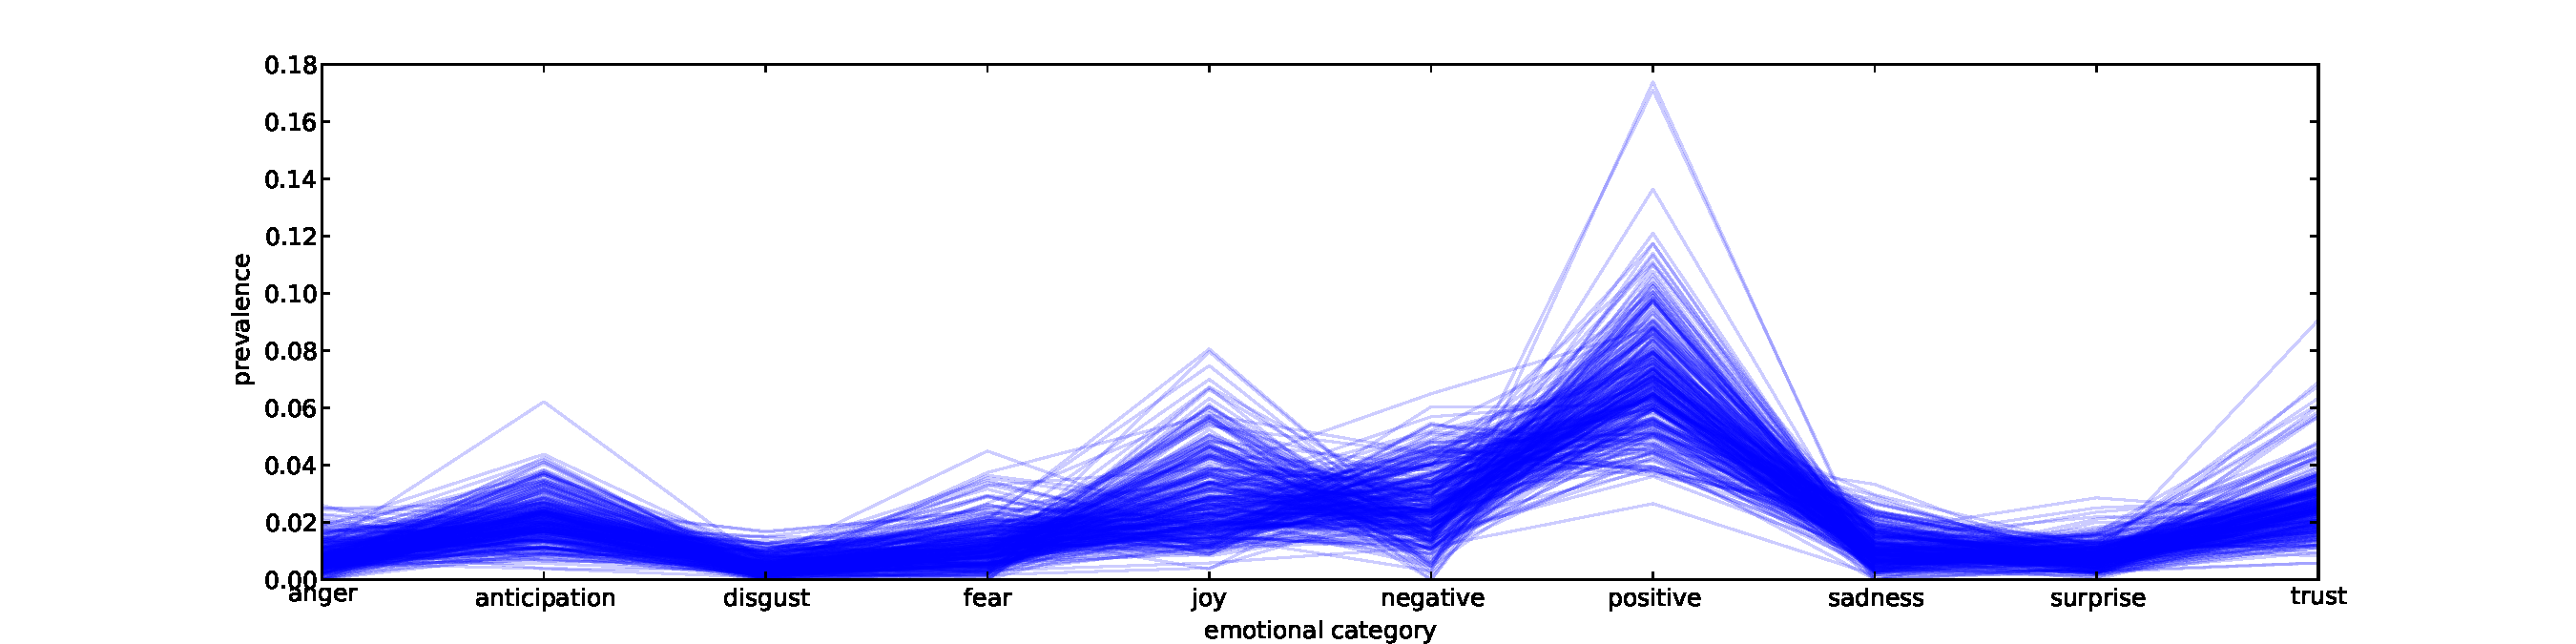
\includegraphics[scale=0.4]{../experiments/exp10.pdf}}
\end{align*}
\end{center}
\vspace{-.6cm}
\caption{A histogram of word distributions of the response for each poem. Here, each poem is represented by one line. The heavy overlap suggests that there is much similarity in the word distribution over comments.}
\vspace{.5cm}
\label{histogram}
\end{figure*}


\subsection{Predicting Proportion of Affect Words}
Next, we aim to characterize the magnitude of affect response, which we quantify with the affect ratio. Multiple poetic features are correlated with the affect ratio, as shown in Table~\ref{feature-correlation}. Notably, the strongest correlated features with $p \le 0.005$ are: HGI-positiv, HGI-concrete, NRC-joy, NRC-trust, NRC-anticipation, type-token ratio, perfect rhyme score, and proportion of stops. When using such features, we are able to predict the affect ratio with 34.6\% reduction in error over simply predicting the average.

\begin{figure*}[ht]
\begin{center}
\begin{align*}
\centerline{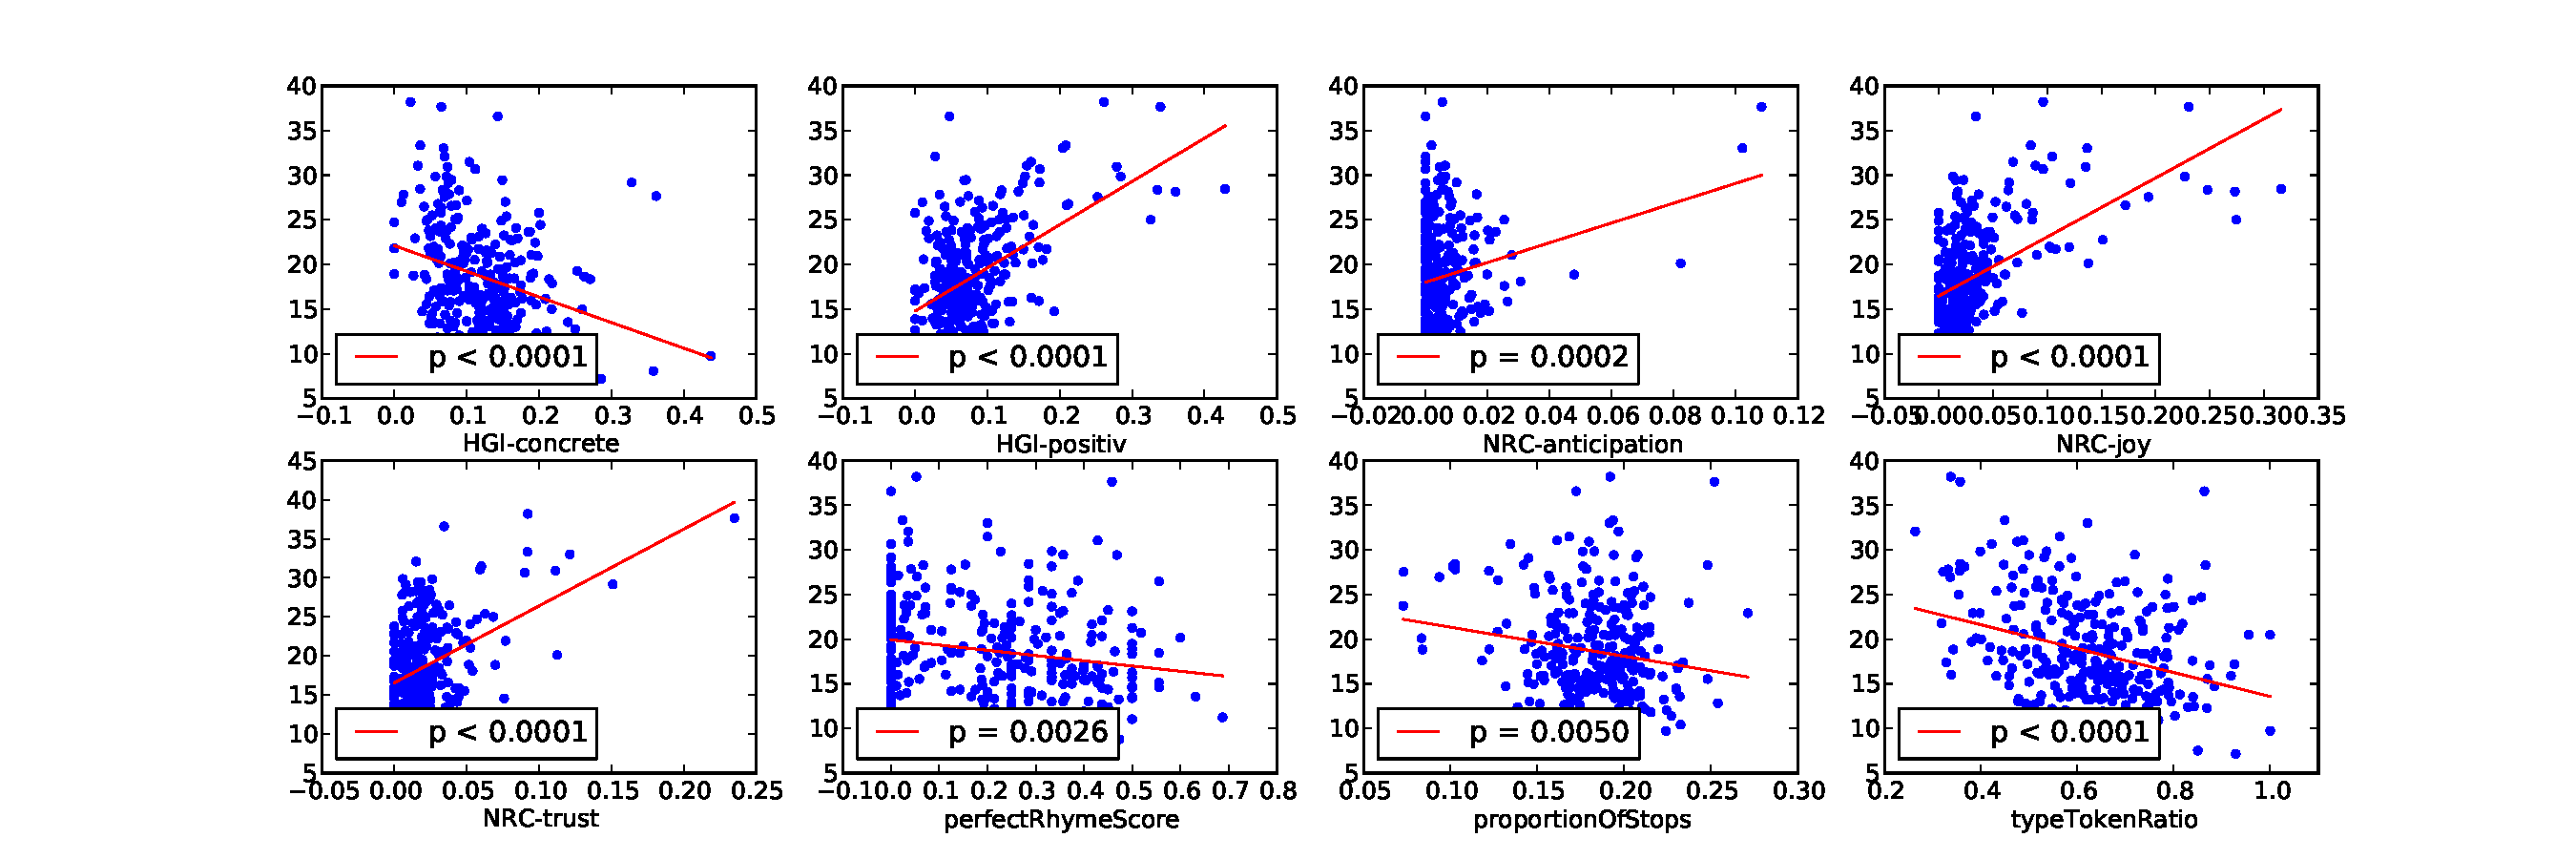
\includegraphics[scale=0.4]{../experiments/affect-ratio.pdf}}
\end{align*}
\end{center}
\vspace{-0.8cm}
\caption{A collection of scatter plots showing the correlation of statistically significant poem features and the comment affect ratio.}
\vspace{0.5cm}
\label{affect-ratio-features}
\end{figure*}


\begin{table*}['ht]
\scriptsize
\begin{center}
\label{feature-correlation}
\vskip 0.12in
\begin{tabular}{l @{\hspace{15pt}} rr @{\hspace{20pt}} rr @{\hspace{20pt}} rr @{\hspace{20pt}} rr @{\hspace{20pt}} rr}
\toprule[.12em]\addlinespace
&\multicolumn{2}{c}{Affect ratio}&\multicolumn{2}{c}{Type-token ratio}&\multicolumn{2}{c}{Avg. comment len.}&\multicolumn{2}{c}{Rating}&\multicolumn{2}{c}{Num. comments}
\\ Feature & correl. & p & correl. & p & correl. & p & correl. & p & correl. & p
\\ \addlinespace \midrule \addlinespace
NRC-joy & $0.51$ & $<0.0001$ & -$0.39$ & $<0.0001$ & -$0.34$ & $<0.0001$ & $0.06$ & $0.1883$ & -$0.07$ & 0.2583
\\ HGI-positiv & $0.51$ & $<0.0001$ & -$0.35$ & $<0.0001$ & -$0.31$ & $<0.0001$ & $0.07$ & $0.1531$ & -$0.10$ & 0.1013
\\ NRC-trust & $0.42$ & $<0.0001$ & -$0.25$ & $<0.0001$ & -$0.29$ & $<0.0001$ & -$0.02$ & $0.6105$ & -$0.11$ & 0.0578
\\ type-token & -$0.32$ & $<0.0001$ & $0.24$ & $<0.0001$ & $0.23$ & $0.0001$ & -$0.14$ & $0.0019$ & $0.02$ & 0.7834
\\ HGI-concrete & -$0.30$ & $<0.0001$ & $0.12$ & $0.0395$ & $0.14$ & $0.0189$ & -$0.07$ & $0.1130$ & $0.01$ & 0.8386
\\ NRC-anticipation & $0.22$ & $0.0002$ & -$0.09$ & $0.1223$ & -$0.15$ & $0.0109$ & -$0.01$ & $0.8357$ & -$0.08$ & 0.1523
\\ perfect rhyme score & -$0.18$ & $0.0026$ & $0.16$ & $0.0075$ & $0.16$ & $0.0080$ & -$0.05$ & $0.3116$ & -$0.09$ & 0.1171
\\ proportion of stops & -$0.16$ & $0.0050$ & $0.18$ & $0.0026$ & $0.18$ & $0.0021$ & $0.03$ & $0.4866$ & $0.11$ & 0.0594
\\ \addlinespace\bottomrule[.12em]
\end{tabular}
\caption{Features most strongly correlated with affect ratio.}
\end{center}
\end{table*}

\subsection{Predicting Average Response Length}
Clearly, there is an identifiable difference in the text of the responses. With the goal of further clarifying this difference, we attempt to predict the average response length. Using the same features as above, we are able to predict this with 15.7\% reduction in error over guessing the average. As observable in Table~\ref{feature-correlation}, the features' correlations with average response length was the opposite of their correlation with average response length. For example, though increased type-token ratio in the poem was correlated with decreased affect ratio, it was also correlated with \emph{increased} comment response length.

\subsection{Predicting Type-Token Ratio}
Additionally, we attempted to predict the type-token ratio of the responses given the poetic features identified as most useful in predicting affect ratio. Feature correlations with type-token ratio were similar to those with average response length, as shown in Table~\ref{feature-correlation}. For example, poem type-token ratio was positively correlated with both average response length and comment type-token ratio. We were able to predict type-token ratio with 17.0\% reduction in error over guessing the average.

\subsection{Predicting Average Rating}
\newcite{kao2012computational} suggest that poem aesthetics can be captured using poetic features. Using public approval as a mark of aesthetic value, one should be able to predict the average poem score using our features. However, we were unable to predict this feature well. This is also expected from Table~\ref{feature-correlation}, which shows that features for this metric did not have both high correlation and low p-value, which also holds for the omitted features.

\subsection{Predicting Number of Comments}
Similarly, one might use the number of comments as a mark of aesthetic value. Increased number of comments could be seen as a mark of increased popularity, or of engendering more discussion. However, we were unable to predict this either.

\section{Discussion and Error Analysis}
In this paper, we drew upon earlier computational work in the analysis of poetry to develop a set of linguistic and poetic features which we then used to predict emotive and linguistic content of the user responses. While predicting emotional word-association distributions proved to be a dead end, we achieved interesting results in predicting the proportion of \emph{affect} words, the average length of comment, and the commentary type-token ratio.

In particular, considering the features that proved to have a statistically significant impact in our prediction tasks, we found that more highly emotive poems (i.e. poems eliciting a higher affect ratio) tend to have strongly distinguished sentiment diction (more positive words, more words associated with \emph{joy}, \emph{trust}, and \emph{anticipation}), fewer concrete words, and a lower type-token ratio.

Among our raw phonetic features, only the proportion of stops proved statistically significant across several of our metrics, a high proportion correlating with a high affect ratio and low type-token ratio. This is at first a finding that is difficult to interpret, but looking at the data we observe that poems with a high proportion of stops tend to be highly repetitive. Therefore, it seems that this ostensibly phonetic feature is most likely encoding one facet of the repetitiveness of the diction, but perhaps a more detailed study focusing on phonetics---perhaps line by line?---could provide a clearer sense of how phonetic components might contribute to emotional response.

Our results appear at first glance to contradict \newcite{kao2012computational}. Kao and Jurafsky found that concrete words and a higher type-token ratio were indicators of poetry written by professionals, as compared with poetry written by amateurs. One might assume that professional poetry is far more likely to produce an emotive response. Finding, then, that within our dataset of opposite trends produced more ``emotive'' poetry per our metrics is a result that requires a more in-depth explanation.

Further examination shows that responses having a high proportion of affect words tend to be shorter than poems with low proportion of affect words. Take, for instance, the following comments with high affect ratio:

\begin{itemize}
\item \emph{what beautiful use of words. lovely poem.}
\item \emph{amazing. maya angelou is the best poet of all time in my opinion.}
\end{itemize}

contrasted with some comments having low affect ratio:

\begin{itemize}
\item \emph{christ's life is plausible. however, consider the theme of ambition: what it is; whether it is neutral or with the power to possess good or evil; and its source. then think to how 'we people on the pavement' took to a person whose skeletons were not on public display.}
\item \emph{this is poetic therapy at its very best. life-changing and liberating. i can't stop reading it...}
\end{itemize}

Indeed, this is a general trend of the comments: the high affect ratio comments tended to be very short ones, as shown in Figure~\ref{affect-ratio-length}. Further analysis shows that affect ratio, log of average comment length, and comment type-token ratio are all strongly correlated with each other. We can offer an interpretation: some comments are very short and offer praise without explanation or justification, and other comments are lengthy, often addressing particular details of the poem.

\begin{figure*}[ht]
\begin{center}
\begin{align*}
\centerline{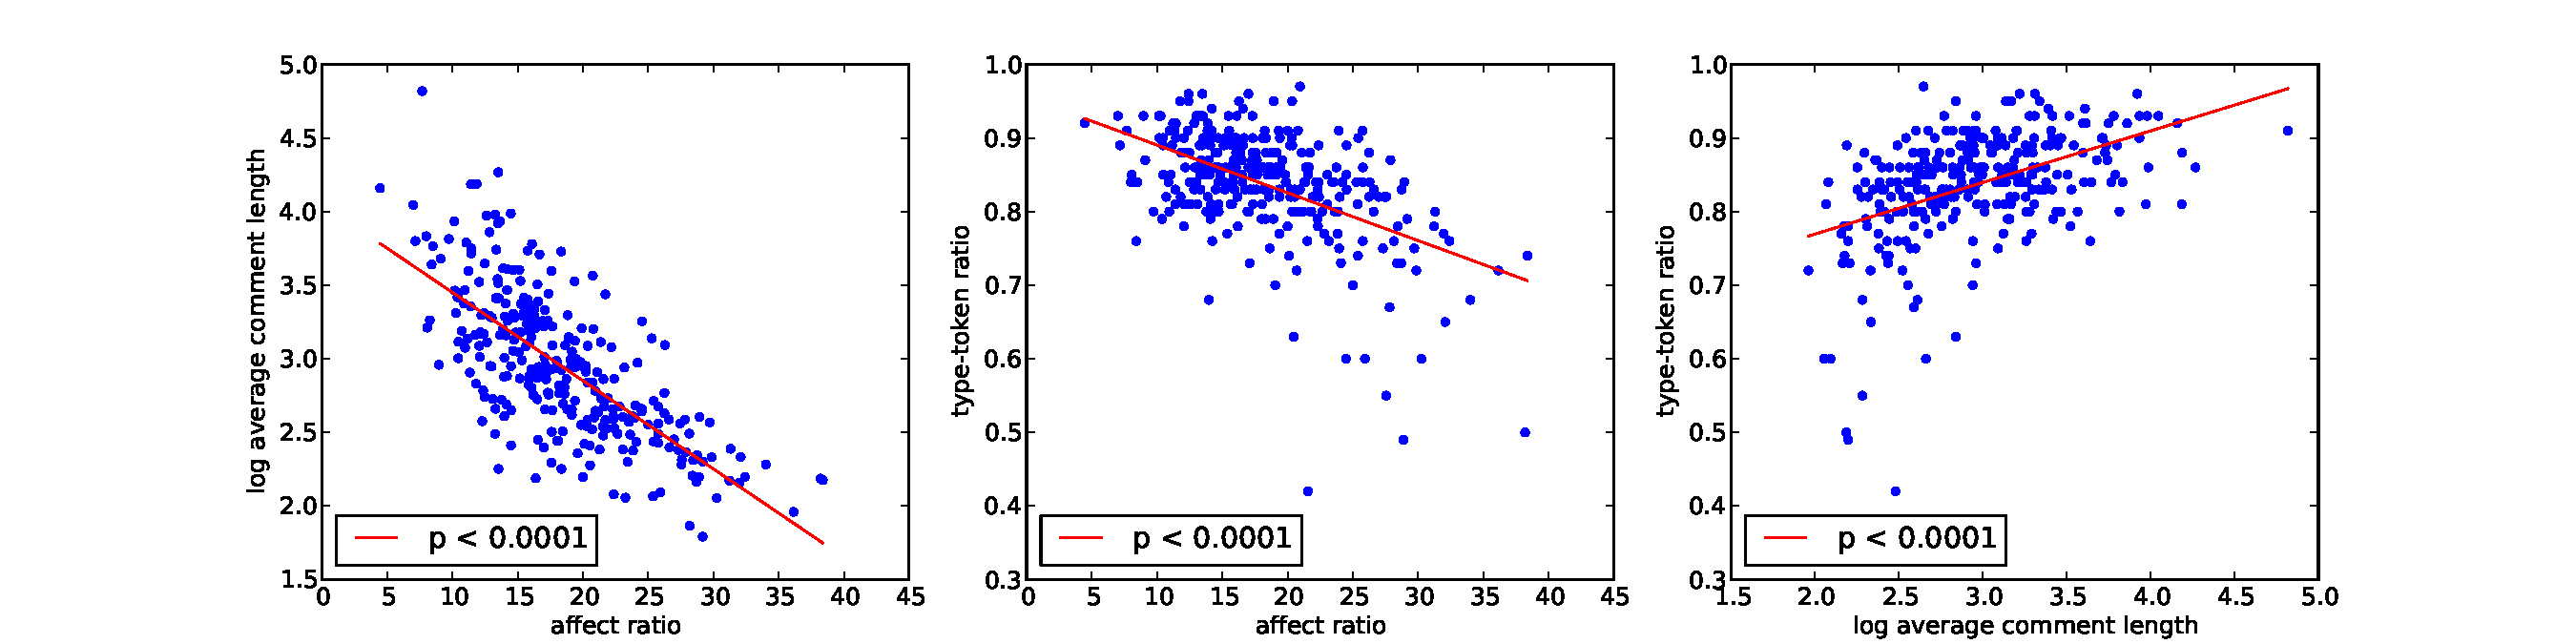
\includegraphics[scale=0.4]{../experiments/exp12.pdf}}
\end{align*}
\end{center}
\caption{A collection of scatter plots for features of the comments, showing the correlations of affect ratio, log average comment length, and comment type-token ratio.}
\label{affect-ratio-length}
\end{figure*}

This result is problematic for our analysis. While we set out to attempt to understand something about how linguistic and poetic features contribute to the production of an emotive response in readers of poetry, we found first that our attempt to predict emotional distributions was unsuccessful, and second that our primary feature for attempting to understand emotional magnitude in the comments---the ratio of affect words---perhaps doesn't represent emotional intensity of the response.

On the contrary, these results complicate our understanding of a text-linguistic approach to emotional response. They raise the question: which indicates a stronger response, a simple ``AMAZING!'' or a lengthy, detailed analysis of a poem's merits, references, and philosophical implications? The answer is unclear because they are qualitatively different \emph{kinds} of responses.

What we can say, however, is that increased complexity in the poem-side featureset (higher type-token ratio, lower perfect rhyme score, less explicitly positive words, and so on) seems to yield increased complexity in the comment responses (higher type-token ratio, longer comments, and a decreased ratio of affect words), and vice versa. Complex poems yield long and complex responses, while simpler poems yield simple, to-the-point responses.

It's worth noting that on the whole this finding does not make any claims about some abstract poem ``quality,'' or whether people like the poem---beyond the finding that lower type-token ratio is associated with higher ratings, our findings predicting poem rating or the number of comments a poem would receive were not statistically significant. 

\section{Future work}

While our model uncovered an interesting positive correlation between the broadly-defined \emph{complexity} of a poem and its responses, we still remain largely in the dark about true \emph{emotiveness}. One issue may be the size of our dataset. An immediate step to address this issue is to expand the dataset. We have already scraped 40,000 additional poems by the top 400 poets on the Top 500 Poets list from the same website. The distribution of comments is very sparse, however. After filtering to only using poems with at least 10 comments in response, we are left with 521 new poems. Upon a brief examination of these new data reveals an average of 11 comments per poem, with an average number of 15 tokens per comment. Recall that the dataset we extracted from the Top 500 Poems has an average of 53 comments per poem, and 20 tokens per comment. It makes sense that Top 500 Poems would receive more comments than all poems written by the Top 500 Poets. It will be interesting to see if, given the discrepancies in data distribution, the results would still be consistent with our current findings.

Other possible methods to get at the real question of emotive response might include a more complex model of comment-side sentiment, richer poem-side features, or a more controlled experimental environment; the text-to-text analysis framework of this study certainly made it difficult to have any sense of ``ground truth'' labels to predict against. Furthermore, the fact that almost all the poems in our dataset are relatively ``canon'' poems from professional poets may result in a relatively uniform (albeit significant) emotional response. 



\section*{Acknowledgments}

Many thanks to our professors Chris Potts and Bill MacCartney for a wonderful quarter, and to our TAs Natalia, Matt, and Kat for their help throughout. Thanks in particular to Chris for his specific suggestions on this project, and for providing us with access to the PragLab account for our preliminary data collection experiments on Mechanical Turk.


\bibliographystyle{acl}
\bibliography{bib}


\end{document}




